\problemname{Staggering to the Finish}

An oval track and field racing track consists of two parallel
straightaway sections connected by two semicircles, depicted in
Figure~1.  Footraces run in the counterclockwise direction, ending at
a common finish line located along the lower straightaway.  For races
that exceed the length of a single straightaway, starting lines must
be staggered backwards, in the clockwise direction, from the finish
line.  The staggered starting lines must account for the curve of the
semicircles and the widths of each running lane.
\begin{figure}[h]
	\begin{center}
		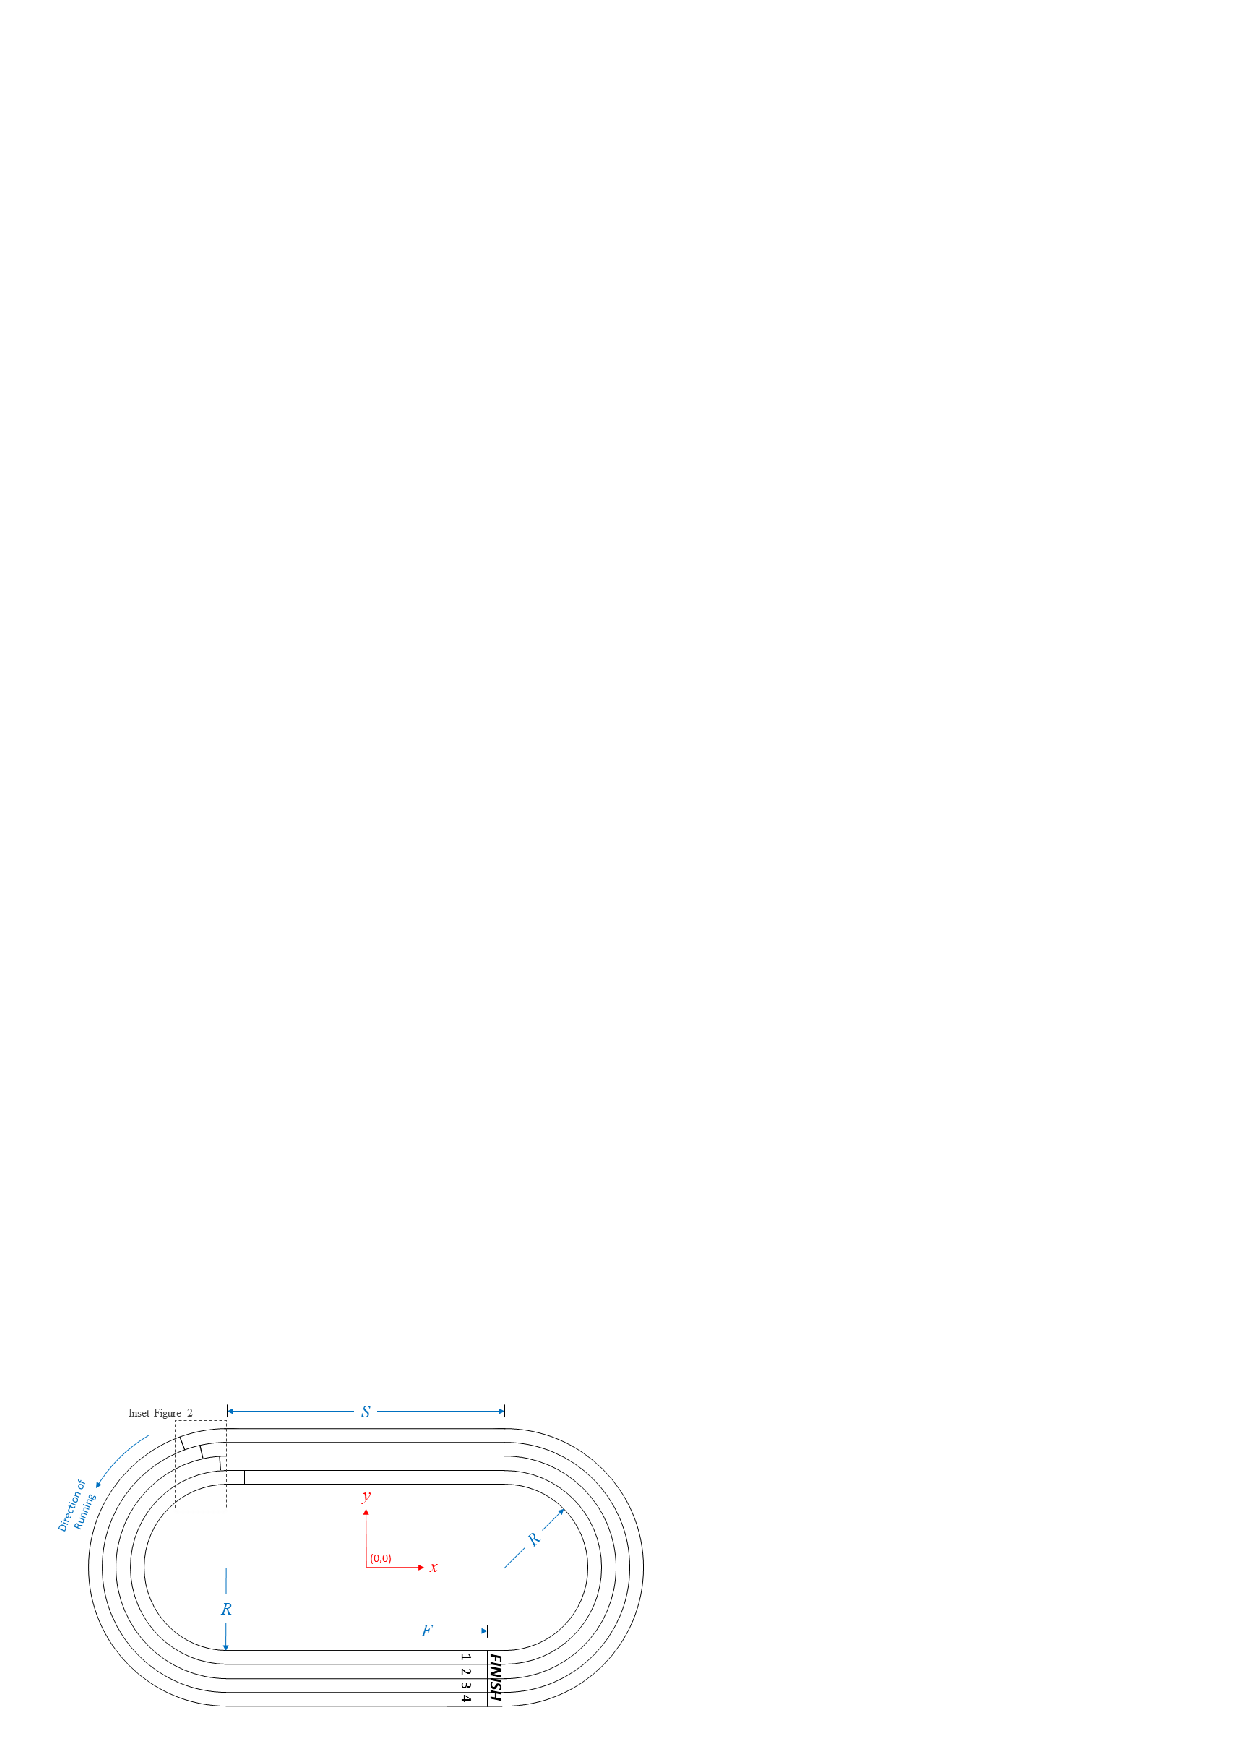
\includegraphics[width=.85\textwidth]{F1Stagger.png}
	\end{center}
\caption{Oval track with $200$m starting lines.}
\end{figure}
\begin{figure}[h]
	\begin{center}
		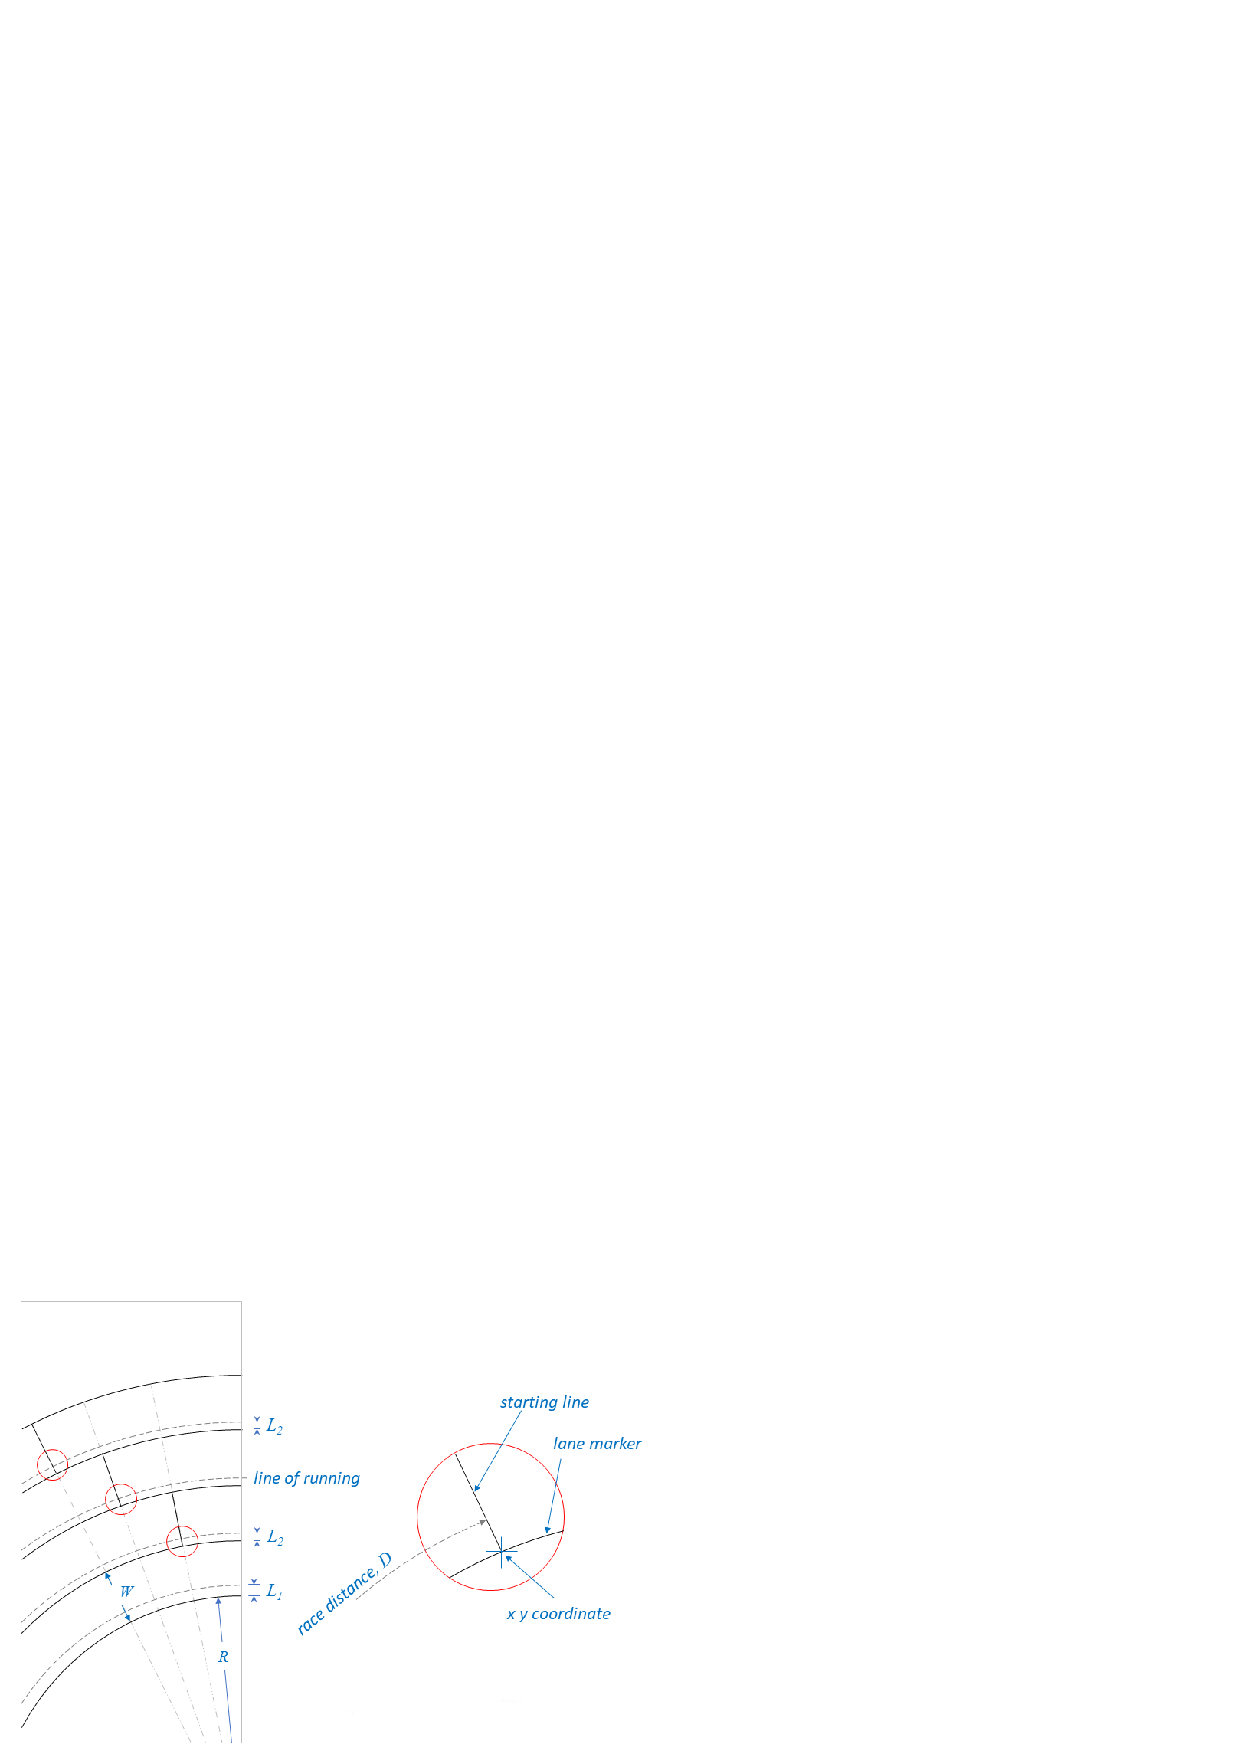
\includegraphics[width=.75\textwidth]{F2Stagger.png}
	\end{center}
\caption{Inset showing staggered starting line locations.}
\end{figure}
\par
There are international standards for oval track dimensions.
Unfortunately, the available area for a track doesn't always hold a
standard track.  Given the dimensions of the track and the length of
the race, your team is to write a program to ensure equal race lengths
by computing the staggered starting line positions.
\par
The total distance of a race for any given lane is computed from the
{\sl line of running}.  The line of running is an unmarked line to
the right of the lane's inside marker (as seen from the
counterclockwise direction).  See Figure~2.  For the innermost lane
(lane 1) the line of running is usually farther from the lane marker
than for the remaining lanes.
% because the inside lane marker is often a raised concrete curb rather
% than a painted line.
\par
The track is mapped to an $(x, y)$ coordinate system with $(0, 0)$ at the
center of the track.  See Figure 1.

\section*{Input}

The first line of input to your program contains seven values,
\hbox{$N$ $R$ $S$ $W$ $F$ $L_1$ $L_2$},
separated by whitespace, describing the geometry of a track, where:
\begin{itemize}
	\item $N$ is the integer number of lanes. ($1 \le N \le 9$)
	\item $R$ is the inner radius of lane 1, a real number in meters.  See Figure~1.  ($1.0 \le R \le 100.0$)
	\item $S$ is the length of the straightaway, a real number in meters.
	See Figure~1.  ($1.0 \le S \le 200.0$)
	\item $W$ is the width of each lane, a real number in meters.
	See Figure~2.  ($0.5 \le W \le 3.0$)
	\item $F$ is the $x$-coordinate of the finish line, measured from the centerline in Figure~1, a real value
	in meters.  The finish line will always be in the lower (negative $y$) half of the track.  ($\vert F\vert \le S / 2$)
	\item $L_1$ is the offset from the inner radius of lane~1 to the line of running for lane~1, a real number in meters.
	See Figure~2.  ($0 \le L_1 < W$)
	\item $L_2$ is the offset from the inner radius to the lines of running for lanes~2 and higher.  See Figure~2.  ($0 \le L_2 < W$)
\end{itemize}
The remaining lines until end-of-file specify $D$, the distance of a race, one race per line, a real number in meters. ($1.0 \le D < 410.0$.) There will be at most $100$ distances $D$ in input.

\section*{Output}

Your program is to print a series of values for each race distance, separated
from each other by spaces and/or newlines.
Print the race distance first, followed by the $(x, y)$ coordinates of the staggered starting line locations in lane number order.
Express all values in
meters.  The $(x, y)$ coordinate is the innermost point of a lane, NOT the line of running.
Treat each lane {\sl marker} (straightaway or radius) as a zero-width line.
International standards require that the values be within $0.001$ meters of
the exact answer.